\documentclass{standalone}

\usepackage{pgfplots}
\usetikzlibrary{calc}
\usetikzlibrary{intersections}
\usetikzlibrary{arrows.meta}
\begin{document}
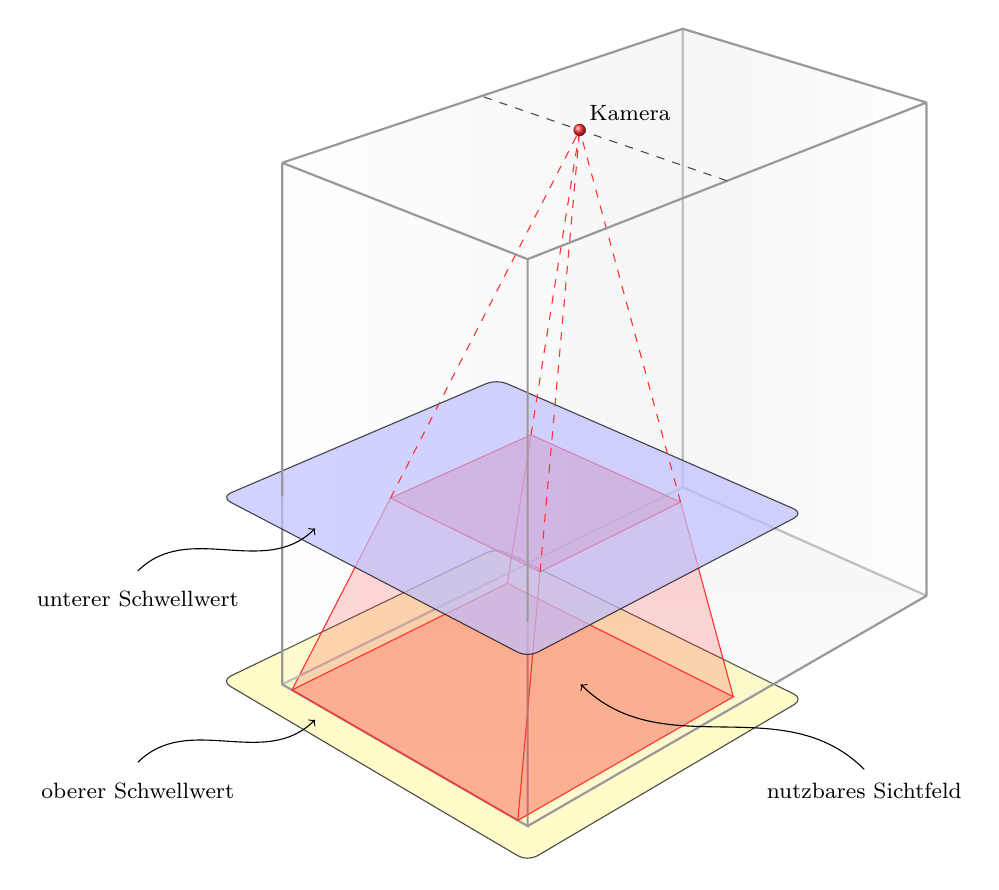
\begin{tikzpicture}[scale=0.9]
        %%% Parameter %%%
        \pgfmathsetmacro{\frameHeight}{8}
        \pgfmathsetmacro{\frameWidth}{0.92}
        \pgfmathsetmacro{\frameDepth}{0.87}
        \pgfmathsetmacro{\viewpointDepth}{0.5}
        \pgfmathsetmacro{\viewpointCentering}{0.6}
        \pgfmathsetmacro{\projectionHeight}{0.36}
        \pgfmathsetmacro{\projectionWidth}{0.96}
        \pgfmathsetmacro{\projectionDepth}{0.07}
        \pgfmathsetmacro{\clippingPlaneHeight}{0.1}
        \pgfmathsetmacro{\clippingPlaneWidth}{0.91}
        %%%%%%%%%%%%
        %%%%%%%%%%%%
            % Fluchtpunkte
        \coordinate (F1) at (30:50cm);
        \coordinate (F2) at (150:50cm);
            % Eckpunkte
        \coordinate (P1) at (0cm,0cm);                  % v U
        \coordinate (P2) at (0cm,\frameHeight);     % v O
        \coordinate (P3) at ($(F1)!\frameDepth!(P1)$);  % h U
        \coordinate (P4) at ($(F1)!\frameDepth!(P2)$);  % h O
        \coordinate (P5) at ($(F2)!\frameWidth!(P1)$);  
        \coordinate (P6) at ($(F2)!\frameWidth!(P2)$);
        \coordinate (P7) at (intersection cs: first line={(P5) -- (F1)}, second line={(P3) -- (F2)});
        \coordinate (P8) at (intersection cs: first line={(P6) -- (F1)}, second line={(P4) -- (F2)});
        \coordinate (P9) at ($(P2)!\viewpointDepth!(P4)$);
        \coordinate (P10) at (intersection cs: first line={(P9) -- (F2)}, second line={(P6) -- (P8)});
            % Sichtfeld
        \coordinate (A) at ($(P5)!\projectionWidth!(P1)$);
        \coordinate (B) at ($(P1)!\projectionWidth!(P5)$);
        \coordinate (C) at ($(A)!\projectionDepth!(F1)$);   
        \coordinate (D) at (intersection cs: first line={(C) -- (F2)}, second line={(B) -- (F1)});  
        \coordinate (V) at ($(P9)!\viewpointCentering!(P10)$);
            % Nutzfläche Schnitt
        \coordinate (E) at ($(A)!\projectionHeight!(V)$);
        \coordinate (F) at (intersection cs: first line={(E) -- (F2)}, second line={(V) -- (B)});
        \coordinate (G) at (intersection cs: first line={(E) -- (F1)}, second line={(V) -- (C)});
        \coordinate (H) at (intersection cs: first line={(F) -- (F1)}, second line={(V) -- (D)});
            % nutz Sichtfeld Ebene
        \coordinate (P11) at (0, \projectionHeight*\frameHeight-0.5);
        \coordinate (P12) at ($(P11)!\clippingPlaneHeight!(F2)$);
        \coordinate (P13) at ($(F1)!\clippingPlaneWidth!(P11)$);
        \coordinate (P14) at at (intersection cs: first line={(P12) -- (F1)}, second line={(P13) -- (F2)});
            % real Sichtfeld Ebene
        \coordinate (P15) at (0, -0.5);
        \coordinate (P16) at ($(P15)!\clippingPlaneHeight!(F2)$);
        \coordinate (P17) at ($(F1)!\clippingPlaneWidth!(P15)$);
        \coordinate (P18) at (intersection cs: first line={(P16) -- (F1)}, second line={(P17) -- (F2)});
            % Hilfspunkte Höhe Ebene
        \coordinate (P19) at (0, \projectionHeight*\frameHeight);
        \coordinate (P20) at ($(F2)!\frameWidth!(P19)$);
        %Linien
        \draw[rounded corners, draw=black, fill=yellow!30, opacity=0.7] (P15) -- (P16) -- (P18) -- (P17)  -- cycle;
            % Tiefe / Verlauf
        \begin{scope}[opacity=0.1]
        \shade[top color=gray!70,bottom color=gray!5] (P1) -- (P3) -- (P7) -- (P5);
        \shade[right color=gray!70,left color=gray!5] (P5) -- (P6) -- (P8) -- (P7);
        \shade[left color=gray!70,right color=gray!5] (P7) -- (P3) -- (P4) -- (P8);
        \end{scope}
            %Frustum
        \begin{scope}[red!80]
            \draw (A) -- (E);
            \draw (B) -- (F);
            \draw (D) -- (H);
            \draw (C) -- (G);
        \end{scope}
            %Frame Unterteil + Hinterteil
        \draw[thick, color=black!25]  (P3) -- (P7) -- (P8)  (P5) -- (P7);
        \draw[thick, color=black!40]  (P20) -- (P5) -- (P1) -- (P19);
            % Sichtfeld der Kamera
        \fill [red!80, opacity=0.3] (A) -- (B) -- (D) -- (C);
        \fill [red!80, opacity=0.4] (E) -- (F) -- (H) -- (G);
        \draw [thin, red!80] (A) -- (B) -- (D) -- (C) -- (A);
        \draw [thin, red] (E) -- (F) -- (H) -- (G) -- (E);
        %\draw [thick, red!80] (
        \begin{scope}[red!80, opacity=0.1]
            \fill (A) -- (B) -- (F) -- (E);
            \fill (C) -- (A) -- (E) -- (G);
            \fill (D) -- (C) -- (G) -- (H);
            \fill (B) -- (D) -- (H) -- (F);
        \end{scope}
        \draw[rounded corners, draw=black, fill=blue!25, opacity=0.7] (P11) -- (P12) -- (P14) -- (P13) -- cycle;
        \begin{scope}[thin, dashed, red!80]%thick, dashed, fill=red!80, opacity=1]
            \draw (E) -- (V);
            \draw (F) -- (V);
            \draw (G) -- (V);
            \draw (H) -- (V);
            %\draw (F1) -- (F3);
            %\draw (F2) -- (F4);
        \end{scope}
            % Frame Oberteil
        \draw[thick,color=black!40] (P19) -- (P2) (P3) -- (P4) (P20) -- (P6)
                                        (P1) -- (P3) (P2) -- (P4) (P2)--(P6) (P6) -- (P8) -- (P4);
        \draw[thin,dashed, color=black!70] (P9) -- (P10);
        % Verbindungspunkte
        \foreach \i in {1,2,..., 10} %20}
            {
             %\shade[shading=ball, ball color=black!80] (P\i) circle (0.05em) node[above right] {}; %\tiny \i};
            }
        \foreach \i in {A, B,...,H}
            {
            %\shade[shading=ball, ball color=red!] (\i) circle (0.05em) node[above right] {}; %\tiny \i};
            }
        %Beschriftung
        %\draw[fill=red] (V) circle (0.25em) node[above right] {\tiny Viewpoint};
        \shade[shading=ball, ball color=red!80] (V) circle (0.25em) node[above right] {\footnotesize Kamera};
        %\draw (-1.1,9.3) node[] {\footnotesize Kamera};
        \draw[thin, -to] (4.75,0.8) to[out=135,in=-45] (0.75,2);
        \draw (4.75,0.5) node[] {\footnotesize nutzbares Sichtfeld};
        \draw[thin, -to] (-5.5,3.6) to[out=45,in=-135] (-3,4.2);
        \draw (-5.5,3.2) node[] {\footnotesize unterer Schwellwert};
        \draw[thin, -to] (-5.5,0.9) to[out=45,in=-135] (-3,1.5);
        \draw (-5.5,0.5) node[] {\footnotesize oberer Schwellwert};
\end{tikzpicture}
\\
\newcommand{\xangle}{7}
\newcommand{\yangle}{138}
\newcommand{\zangle}{90}

\newcommand{\xlength}{1}
\newcommand{\ylength}{1}
\newcommand{\zlength}{1}

\pgfmathsetmacro{\xx}{\xlength*cos(\xangle)}
\pgfmathsetmacro{\xy}{\xlength*sin(\xangle)}
\pgfmathsetmacro{\yx}{\ylength*cos(\yangle)}
\pgfmathsetmacro{\yy}{\ylength*sin(\yangle)}
\pgfmathsetmacro{\zx}{\zlength*cos(\zangle)}
\pgfmathsetmacro{\zy}{\zlength*sin(\zangle)}

\pgfmathsetmacro{\posalongpath}{0.37}
\pgfmathsetmacro{\vertexheight}{8}
\pgfmathsetmacro{\dblength}{1}

\begin{tikzpicture}[x={(\xx cm,\xy cm)}, y={(\yx cm,\yy cm)}, z={(\zx cm,\zy cm)}]
    \coordinate (A) at (0,0,0);
    \coordinate (B) at (3,0,0);
    \coordinate (C) at (3,3,0);
    \coordinate (D) at (0,3,0);
    \coordinate (V) at (2,2,\vertexheight);
    
    \node[above] at (V) {Spacecraft};

    \path (A) -- (V) coordinate[pos=\posalongpath] (A-V);
    \path (B) -- (V) coordinate[pos=\posalongpath] (B-V);
    \path (C) -- (V) coordinate[pos=\posalongpath] (C-V);
    \path (D) -- (V) coordinate[pos=\posalongpath] (D-V);

    \pgfmathsetmacro{\blueheight}{\posalongpath*\vertexheight}

    \coordinate (A1) at ($(A-V) + (0,0,-\blueheight)$);
    \coordinate (B1) at ($(B-V) + (0,0,-\blueheight)$);
    \coordinate (C1) at ($(C-V) + (0,0,-\blueheight)$);
    \coordinate (D1) at ($(D-V) + (0,0,-\blueheight)$);

    \fill[red,opacity=0.5,draw=red!80!black,thick] (A) -- (B) -- (C) -- (D) -- cycle;

    % \fill[yellow,opacity=0.5,draw=red!80!black,thick] (A1) -- (B1) -- (C1) -- (D1) -- cycle;

    \draw[red!50!black] (A) -- (A-V) (B) -- (B-V) (C) -- (C-V) (D) -- (D-V);
    % \draw[blue!50!yellow,densely dashed] (A1) -- (A-V) (B1) -- (B-V) (C1) -- (C-V) (D1) -- (D-V);

    \fill[blue,opacity=0.5,draw=blue!80!black,thick] (A-V) -- (B-V) -- (C-V) -- (D-V) -- cycle; 

    \draw[red!50!black,densely dashed] (V) -- (A-V) (V) -- (B-V) (V) -- (C-V) (V) -- (D-V);

    \fill[red,opacity=0.2] (A) -- (B) -- (B-V) -- (A-V) -- (D-V) -- (D) -- cycle;

\end{tikzpicture}
\\
\begin{tikzpicture}
    \pgfmathsetmacro{\distance}{6};
    \pgfmathsetmacro{\nearplane}{0.37};
    \pgfmathsetmacro{\blueheight}{\nearplane*\vertexheight};
    \pgfmathsetmacro{\hfov}{15};
    \pgfmathsetmacro{\wfov}{15};
    \pgfmathsetmacro{\H}{\distance*tan(\hfov/2)};
    \pgfmathsetmacro{\W}{\distance*tan(\wfov/2)};
    \pgfmathsetmacro{\dlength}{1};

    \pgfmathsetmacro{\conex}{1};
    \pgfmathsetmacro{\coney}{0};
    \pgfmathsetmacro{\conez}{0};

    \pgfmathsetmacro{\ctwox}{0};
    \pgfmathsetmacro{\ctwoy}{1};
    \pgfmathsetmacro{\ctwoz}{0};

    \pgfmathsetmacro{\cthreex}{0};
    \pgfmathsetmacro{\cthreey}{0};
    \pgfmathsetmacro{\cthreez}{1};
    
    \coordinate (V) at (0,0,0);
    \coordinate (A) at ($ (\distance * \conex, \distance * \coney, \distance * \conez) + (-\W * \ctwox, -\W * \ctwoy, -\W * \ctwoz) + ( \H * \cthreex, \H * \cthreey, \H * \cthreez) $);
    \coordinate (B) at ($ (\distance * \conex, \distance * \coney, \distance * \conez) + (\W * \ctwox, \W * \ctwoy, \W * \ctwoz) + ( \H * \cthreex, \H * \cthreey, \H * \cthreez) $);
    \coordinate (C) at ($ (\distance * \conex, \distance * \coney, \distance * \conez) + (\W * \ctwox, \W * \ctwoy, \W * \ctwoz) + ( -\H * \cthreex, -\H * \cthreey, -\H * \cthreez) $);
    \coordinate (D) at ($ (\distance * \conex, \distance * \coney, \distance * \conez) + (-\W * \ctwox, -\W * \ctwoy, -\W * \ctwoz) + ( -\H * \cthreex, -\H * \cthreey, -\H * \cthreez) $);

    \coordinate (m1) at ($ (V) + (\dlength * \conex, \dlength * \coney, \dlength * \ctwoz )$);
    \coordinate (m2) at ($ (V) - (\dlength * \conex, \dlength * \coney, \dlength * \ctwoz )$);

    \path (A) -- (V) coordinate[pos=\posalongpath] (A-V);
    \path (B) -- (V) coordinate[pos=\posalongpath] (B-V);
    \path (C) -- (V) coordinate[pos=\posalongpath] (C-V);
    \path (D) -- (V) coordinate[pos=\posalongpath] (D-V);
    
    % labels of points
    \node[below] at (A) {$A$};
    \node[above] at (B) {$B$};
    \node[above] at (C) {$C$};
    \node[right] at (D) {$D$};

    \draw[red!50!black, dashed] (V) -- (A-V) (V) -- (B-V) (V) -- (C-V) (V) -- (D-V);
    % \draw[red!50!black] (A) -- (A-V) (B) -- (B-V) (C) -- (C-V) (D) -- (D-V);
    \draw[red!50!black, -Latex] (A-V) -- (A);
    \draw[red!50!black, -Latex] (B-V) -- (B);
    \draw[red!50!black, -Latex] (C-V) -- (C);
    \draw[red!50!black, -Latex] (D-V) -- (D);
    \fill[red,opacity=0.5,draw=red!80!black,thick] (A) -- (B) -- (C) -- (D) -- cycle;
    \fill[blue,opacity=0.5,draw=blue!80!black,thick] (A-V) -- (B-V) -- (C-V) -- (D-V) -- cycle; 
    
    \draw[blue!50!black, ultra thick] (m1) -- (m2);
    \shade[ball color=blue] (m1) circle (0.2);
    \shade[ball color=blue] (m2) circle (0.2);

\end{tikzpicture}
\end{document}
